% !Mode:: "TeX:UTF-8"
% !TEX root = ..\thesis.tex
\chapter{研究对象基本情况}
本文以某汽车电子有限公司的装配车间为研究对象,进行调研。本章将介绍该公司车间的基本情况,并对现有装配线调度情况进行初步分析。
\section{公司基本情况}
该汽车电子有限公司主要产品为车用电子电器开关、控制模块、控制面板等,是美国通用、德国大众、一汽大众、上海大众、上海通用、上海汽车、长安福特、北京现代、一汽轿车、奇瑞汽车、哈飞集团等国内外40余家汽车主机厂的专业定点配套供应商,配套的代表性车型有奥迪A6(L)、奥迪A4(L)、奥迪Q5、迈腾、君越、宝来、帕萨特、奔腾、红旗、马自达M6、景程、荣威、明锐、凯越、捷达、桑塔纳等系列轿车,以及卡车、轻型车、微型车等,产品型号达6000余种。

\section{装配车间作业}
该公司的制造部分为制造一部和制造二部,制造一部主要是负责零部件的生产,不是本课题的主要研究对象;制造二部主要是负责产品总装,共8个车间,均是流水线作业,是本课题的研究对象,其相关信息如\reft{tab:2jobshopinfo}所示(单位:个)。
\begin{table}[htbp]
  \centering
  \caption{制造二部装配车间信息}
    \begin{tabular}{cccccccccc}
    \toprule
    \multicolumn{2}{c}{车间 } & 1车间   & 2车间   & 3车间   & 4车间   & 5车间   & SGM车间 & 通用车间  & 电子车间 \footnote{包括:模块线、插件线及SMT线三个部分,其中,模块线是总装线,共5条装配线,插件线和SMT线是零部件生产线。本次研究的重点是总装线,故电子车间只列出了部分信息。} \\
    \midrule
    \multicolumn{2}{c}{班 组 数 量} & 6     & 6     & 6     & 5     & 4     & 4     & 6     & 2 \\
    \multicolumn{2}{c}{流水线数量} & 7     & 7     & 7     & 6     & 7     & 6     & 5     & 5 \\
    \multicolumn{2}{c}{PMC分配品种数} & 777   & 557   & 186   & 196   & 334   & 29    & 76    & 83 \\
    \bottomrule
    \end{tabular}
  \label{tab:2jobshopinfo}
\end{table}

由\reft{tab:2jobshopinfo}可知,每个总装车间均有多条生产流水线,每条流水线负责各自对应主机厂的装配生产。当主机厂需要多个品种的产品时,流水线根据订单顺序进行装配作业,即同一主机厂的产品在一条生产线上轮流生产。

该公司采用面向订单生产,订单从接受到交付的流程如\reff{fig:orderflow}所示,其中虚线框内为装配车间的作业。在没有订单或者订单较少时,为了不让生产线停下来,需要进行工厂内部的计划生产,而订单较多时需要加班作业。
\begin{figure}[h]
\centering
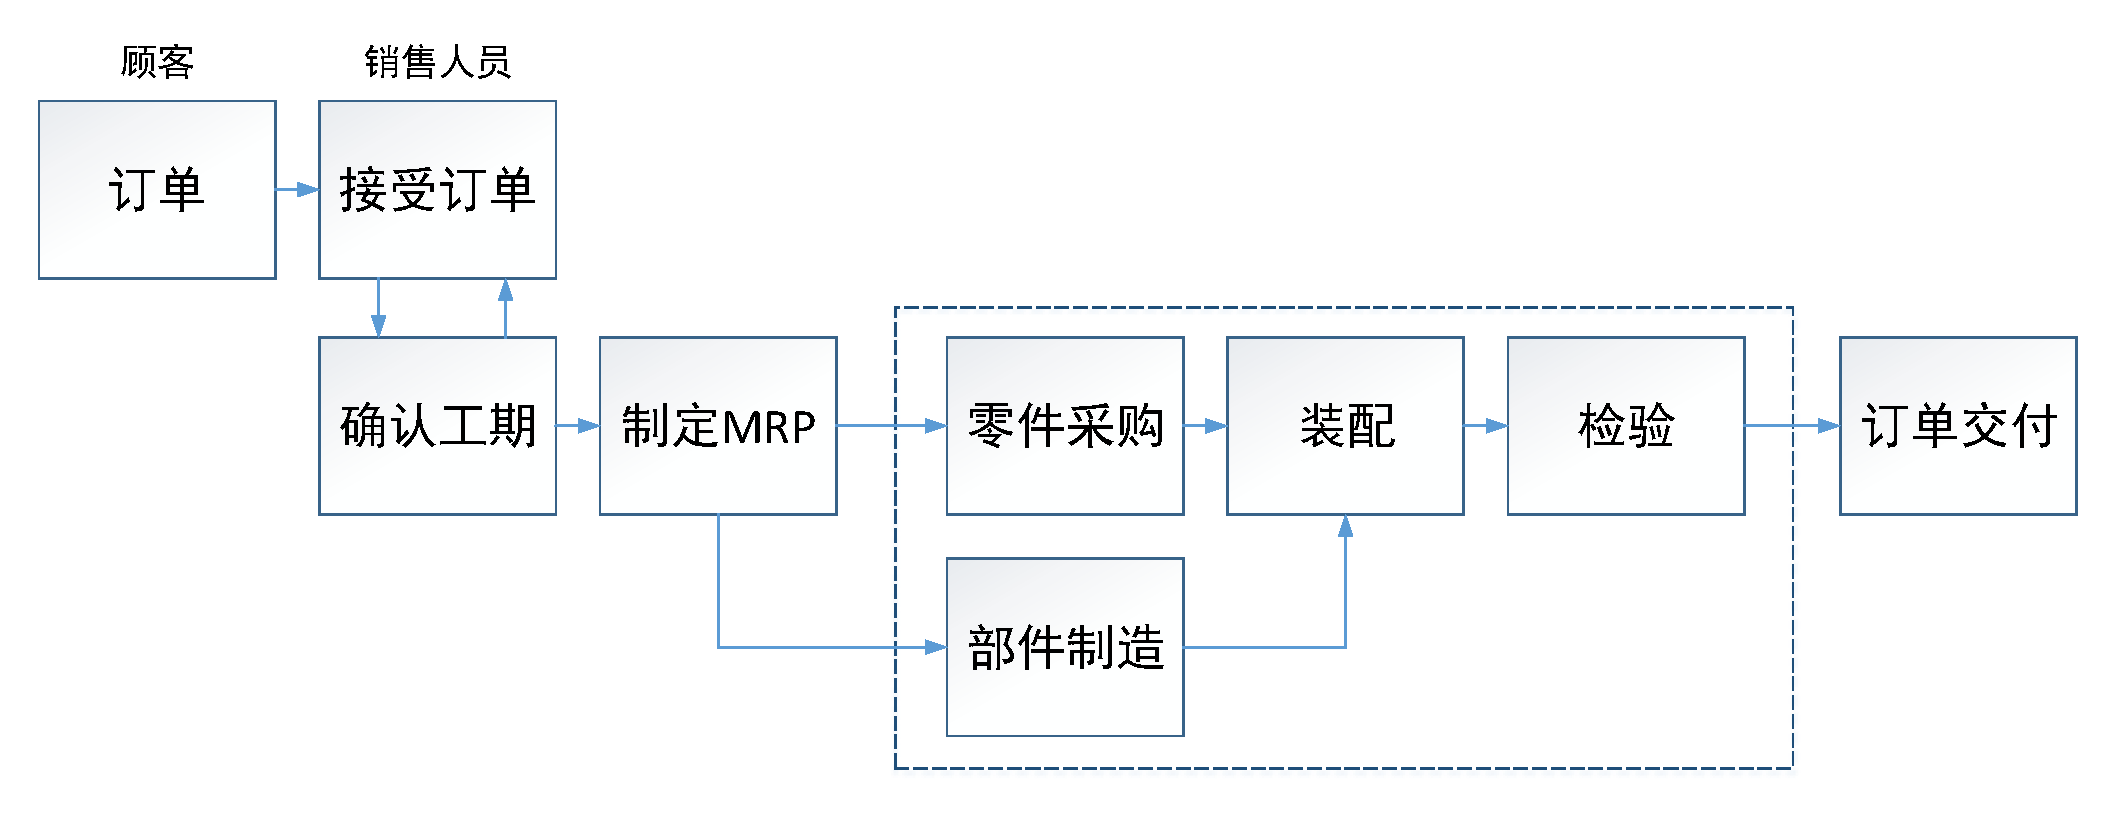
\includegraphics[width = 13cm]{orderflow.pdf}
\caption{现行订单信息流\label{fig:orderflow}}
\end{figure}

\section{产线调度现状}
当前该公司装配车间采用专线生产的方式,即客户的订单在其专用的流水线上进行生产作业,当同一客户有多个订单下达时,按照先到先服务(FCFS)的规则进行装配生产安排,多条产线并行作业互不干扰。

订单或任务到达时,如果有流水生产线空闲可用,则立马对其根据进行生产准备,然后开始装配生产。若产线在处理订单,那么将该订单安排入其专线队列中,等待前面的批量订单生产完毕再进行生产。现行调度的产线如\reff{fig:3nowschedule}所示。

\begin{figure}[h]
\caption{3条生产线的现行调度\label{fig:3nowschedule}}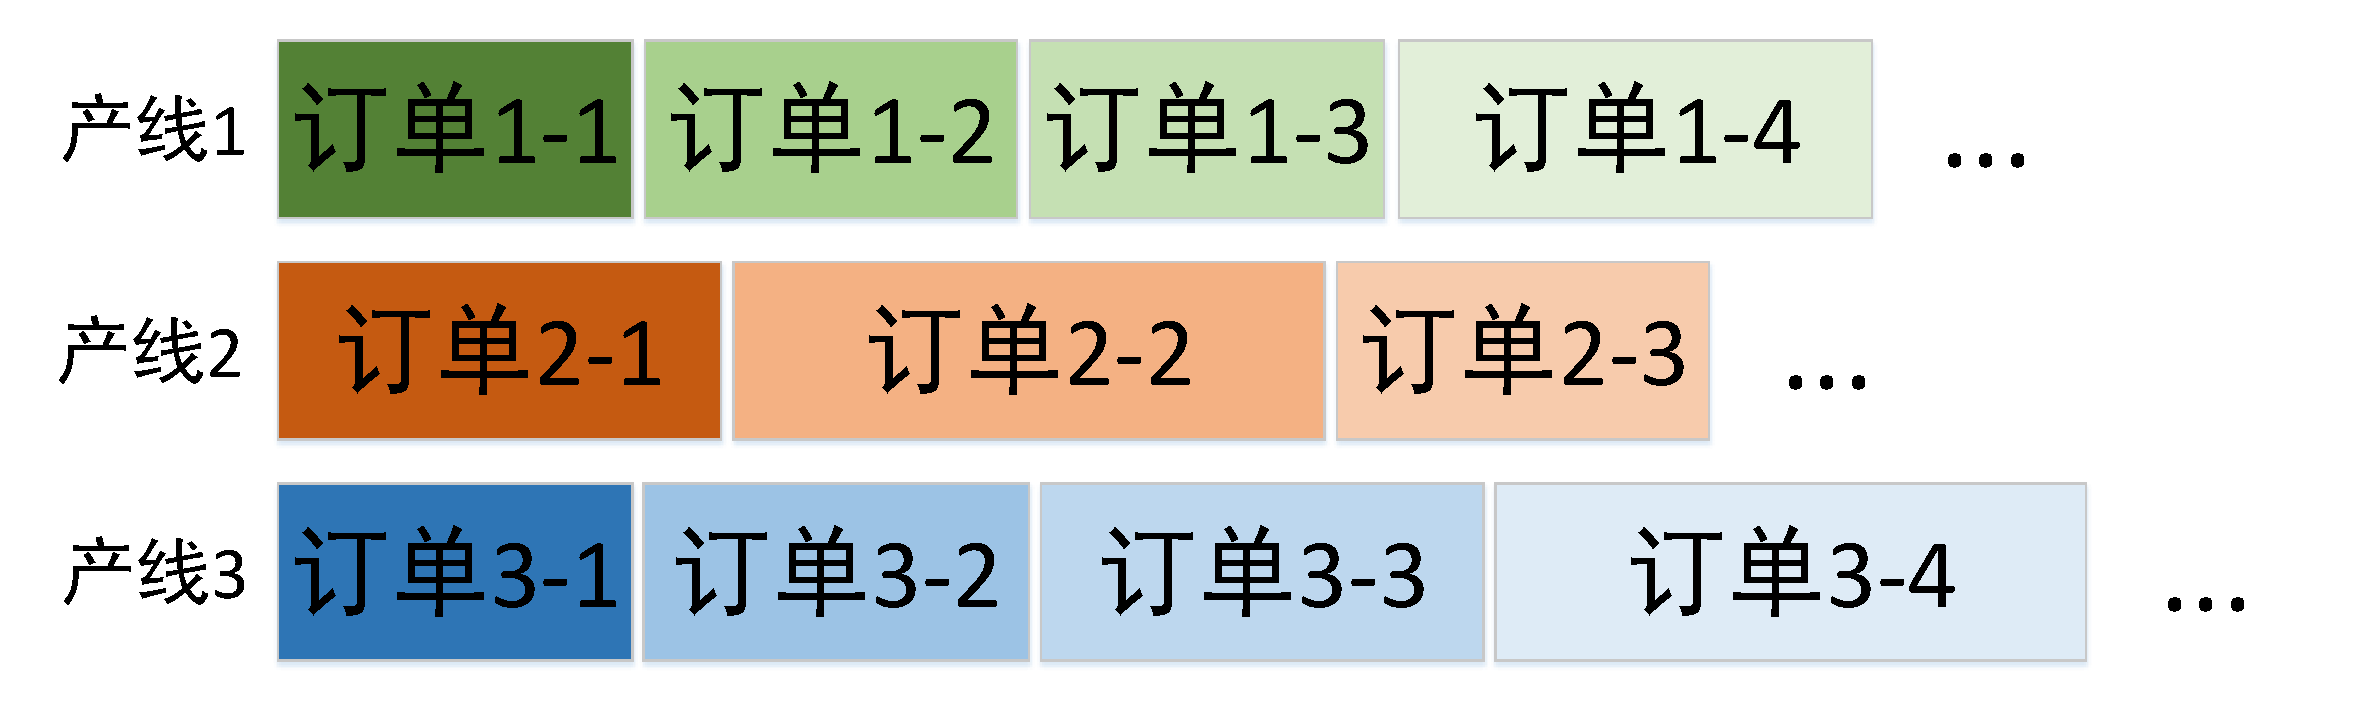
\includegraphics[width = 8cm]{orderschedulenow.pdf}
\end{figure}

现行调度方法逻辑简单,执行力强,每条装配线可分时生产不同品种的产品,而且按照厂家来安排组织生产,方便了管理。然而其缺陷也是明显的,例如常常会产生有些产线队列很长而有限产线空闲无作业,造成极大浪费。具体的现有问题将在下一章分析。
\section{小结}
本章...
产线调度现状反映了一些问题,例如
